
% ------------------------------------------------------------
% ------------------------------------------------------------

%%%%%%%%%%%%%%%%%%%%%%%%%%%%%%%%%%%%%
\section{3D Plots}
\subsection{\ttfamily lattice \normalfont library}
%\begin{frame}
%\frametitle{3D Plots}

%		- lattice, plot3d ...\\
%		- changing plotting options \\
%		- contourplot, wireframe, levelplot \\
%		-rgl, scatterplot3d \\
%		
%\end{frame}

%%%%%%%%%%%%%%%%%%%%%%%
\begin{frame}[fragile]
\title{3D Images}

One way to create 3D images is with the package \ttfamily lattice: \normalfont 

    \begin{columns}
      \column{0.50\textwidth}
\bf{Method 1:} \normalfont Using \ttfamily wireframe(): \normalfont 
\begin{lstlisting}
library(lattice)
wireframe(volcano, color.palette = terrain.colors, asp = 1, color.key=TRUE, drape=TRUE, scales = list(arrows = FALSE))
\end{lstlisting}
%g <- expand.grid(x = 1:10, y = 5:15)
%g$z<-g$x^2
%wireframe(g$z~g$x*g$y, scales = list(arrows = FALSE), drape = TRUE, colorkey = TRUE)

     \column{0.50\textwidth}
       \begin{center}
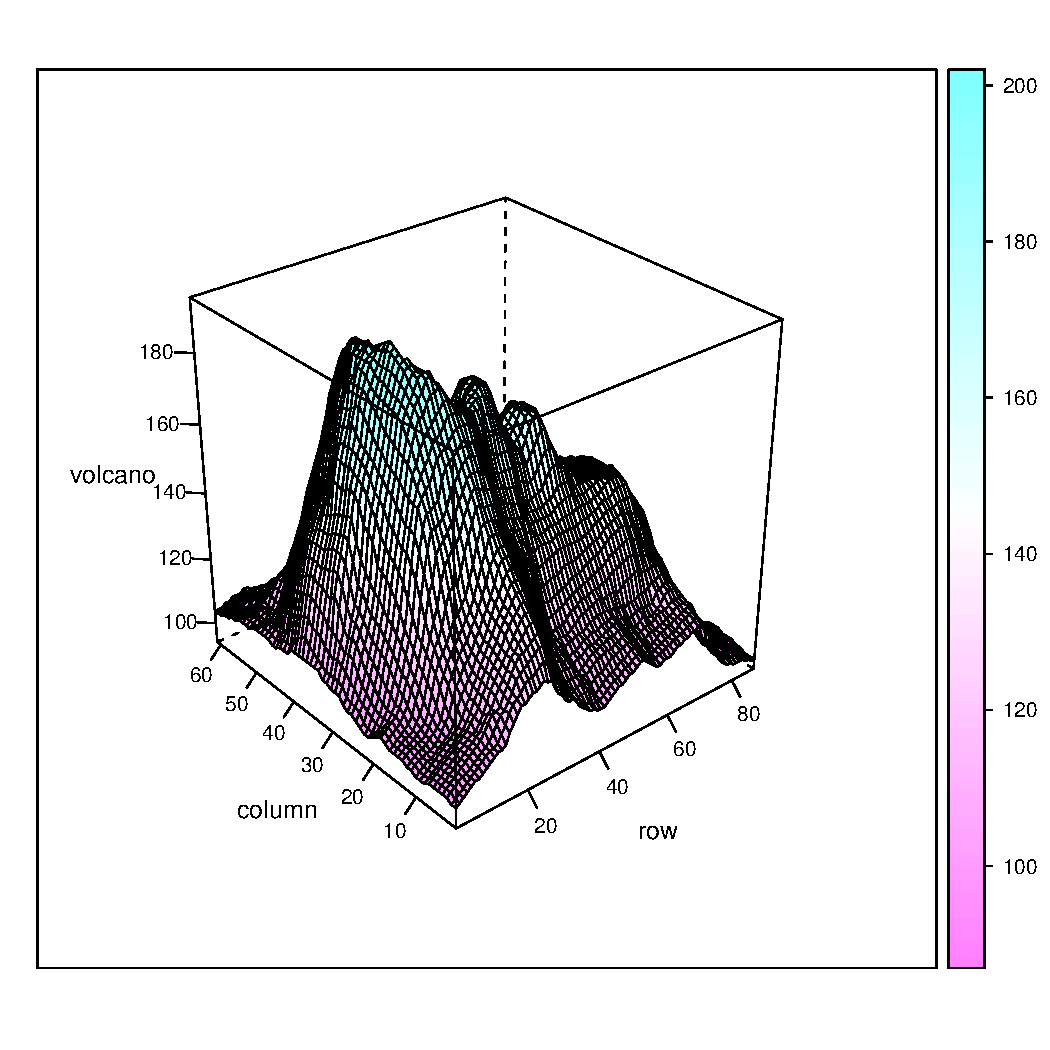
\includegraphics[width = 55mm]{images/wireframe.pdf}
\end{center}
\end{columns}
\end{frame}

%%%%%%%%%%%%%%%%%%%%%%%
\begin{frame}[fragile]
\title{3D Images}

    \begin{columns}
      \column{0.50\textwidth}
\bf{Method 2:} \normalfont Same image with the \ttfamily levelplot(): \normalfont 

\begin{lstlisting}
library(lattice)
levelplot(volcano, color.palette = terrain.colors, asp = 1, color.key=TRUE, drape=TRUE, scales = list(arrows = FALSE))
contour(volcano, add=TRUE, lwd=1.3, labcex=1.3)
\end{lstlisting}

     \column{0.50\textwidth}
       \begin{center}
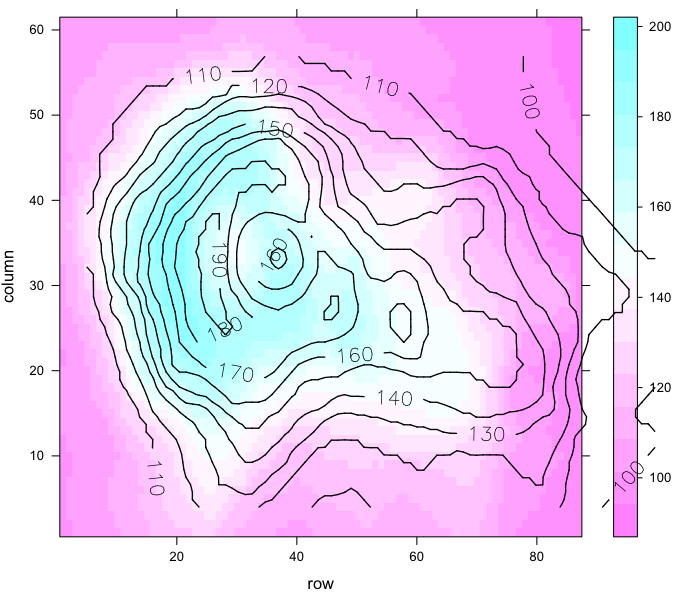
\includegraphics[width = 55mm]{images/levelplot.png}
\end{center}
\end{columns}
\end{frame}
% plot3d(iris)

%%%%%%%%%%%%%%%%%%%%%%%
\subsection{\ttfamily rgl \normalfont library} 
%%%%%%%%%%%%%%%%%%%%%%%
\begin{frame}[fragile]
\title{3D Images}

Another way to create 3D images is with the package \ttfamily rgl: \normalfont 

    \begin{columns}
      \column{0.50\textwidth}
\begin{lstlisting}
library(rgl)
data(quakes)
plot3d(x=quakes[, 2], y=quakes[, 1], z=quakes[, 3], xlab="Longitude", ylab="Latitude", zlab="Depth")
\end{lstlisting}
%g <- expand.grid(x = 1:10, y = 5:15)
%g$z<-g$x^2
%wireframe(g$z~g$x*g$y, scales = list(arrows = FALSE), drape = TRUE, colorkey = TRUE)

     \column{0.50\textwidth}
       \begin{center}
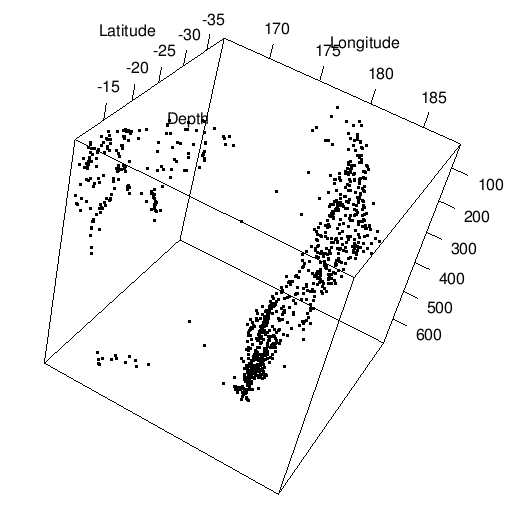
\includegraphics[width = 55mm]{images/Fiji_RGL}
\end{center}
\end{columns}
\end{frame}


% ------------------------------------------------------------
% ------------------------------------------------------------
